\chapter{Fundamentos Teóricos}
\label{cap:theory}

Este capítulo apresentará uma visão geral dos fundamentos teóricos que permitiram a implementação da biblioteca cliente HTTP/2 em Lua. Conceituar o HTTP/2 e a linguagem Lua é de suma importância para sustentar as ideias da implementação. Para isso, o capítulo foi organizado em duas seções: uma seção dedicada à descrição do protocolo HTTP/2 e outra à linguagem Lua. Tanto o HTTP/2 quanto Lua são assuntos naturalmente extensos e portanto cada seção consiste de um breve resumo de conceitos que foram pertinentes à escrita da implementação.

A seção \ref{sec:http2} apresenta uma breve história do HTTP/2 e a natureza dos problemas de desempenho presentes no HTTP, destacando o escopo desses problemas, como eles se manifestam e como estudos passados tentaram resolvê-los. Depois, um breve resumo do protocolo HTTP/2 é apresentado. A completa definição do HTTP/2 é um produto dos RFCs 7540 \cite{BelsheRFC7540} e 7541 \cite{BelsheRFC7541} e podem ser consultados para informações mais detalhadas do protocolo.

A seção \ref{sec:lua} apresenta as principais características da linguagem de programação Lua, juntamente com as bibliotecas escritas em Lua que permitiram uma implementação compatível com a natureza de um cliente HTTP/2. Como a implementação da biblioteca foi feita em Lua, essa seção destaca os principais paradigmas e construções da linguagem que viabilizaram a escrita da biblioteca. Todos os aspectos da linguagem Lua são cobertos pelo livro Programming in Lua \cite{Ierusalimschy2016PiL}.

%% - - - - - - - - - - - - - - - - - - - - - - - - - - - - - - - - - - -
\section{HTTP/2}
\label{sec:http2}

O {\em Hypertext Transfer Protocol version 2} (HTTP/2) é um protocolo da camada de aplicação sem estado de requisição/resposta para sistemas de informação hipertextos, distribuídos e colaborativos definido pelos RFCs 7540 \cite{BelsheRFC7540} e 7541 \cite{BelsheRFC7541}. O RFC 7540 especifica uma nova sintaxe para o HTTP/2, mas não altera a semântica já existente do HTTP/1.1 e o RFC 7541 define um formato de compressão para campos de cabeçalhos HTTP/2.

Um dos propósitos pelo qual a especificação do HTTP/2 foi criada é o de proporcionar um melhor desempenho às aplicações Web ao permitir que clientes e servidores HTTP/2 façam um uso mais eficiente da conexão TCP \cite{Brylinski:2017:OH:3018896.3065841}, onde toda conexão é persistente e as requisições podem ser feitas de forma concorrente. No HTTP/1.1, clientes e servidores têm a opção de usar conexões persistentes ou não persistentes. Porém, quando conexões persistentes são usadas no HTTP/1.1, cada requisição é feita de forma sequencial, ou seja, requisições devem esperar por cada resposta do servidor.

Para que as requisições não precisem esperar por cada resposta, o HTTP/1.1 permitiu paralelismo ({\em pipelining}) de requisições, mas uma requisição que necessita de um processamento significativo no lado do servidor pode resultar em uma resposta grande e lenta, podendo bloquear outras requisições. Esse problema é conhecido como bloqueio de cabeça de fila (HOL -- {\em head-of-the-line blocking}) \cite{Kurose:2012:CNT:2584507}. Além disso, alguns servidores e intermediários não implementam paralelismo corretamente, ao ponto dos principais navegadores em uso atualmente terem desabilitado {\em pipelining} por padrão.

Embora na prática um número significativo de conexões TCP com o servidor podem existir \cite{Manzoor7818414}, realizar um número reduzido de conexões TCP conexões é uma prática importante para diminuir o impacto negativo que o HTTP e o HTTPS têm sobre a rede. Por exemplo: o tempo de viagem de ida e volta ({\em round-trip time} -- RTT) de pacotes de rede é reduzido porque a apresentação de três vias do TCP não precisa ser renegociada depois que cada requisição termina; menos pacotes são enviados na rede; existem menos chances do pacote SYN do TCP ser perdido; o reuso de uma sessão TLS é melhorado e menos {\em handshakes} TLS são feitos. Além disso, usar muitas conexões injustamente monopoliza recursos de rede por parte dos navegadores, por exemplo.

Um segundo propósito pelo qual o HTTP/2 foi criado está relacionado a composição das mensagens HTTP: campos de cabeçalhos redundantes e repetitivos (alguns com tamanho consideravelmente grande) são enviados pela conexão TCP em texto simples. Essa prática causa um tráfego de rede desnecessário e uma rápida negação do controle de congestionamento do TCP, levando a eventos de congestionamento e de retransmissão que prejudicam não só a aplicação, mas a rede como um todo.

O terceiro propósito da criação especificação do HTTP/2 refere-se a preservação da compatibilidade com os atuais usos do HTTP/1.1. Com o intuito de interoperar com a Web existente, o HTTP/2 destina-se a ser tão compatível quanto possível com o HTTP/1.1. Isso significa que, pela perspectiva da aplicação, as características do HTTP/1.1 foram em grande parte inalteradas. Os desenvolvedores não precisam modificar conteúdos de seus sites e as mesmas APIs do HTTP/1.1 ainda podem ser utilizadas.

Para alcançar isso, todas as semânticas de requisição e resposta do HTTP/1.1 \cite{FieldingRFC7231} foram preservadas, mas uma nova sintaxe foi proposta para o HTTP/2. Apesar da semântica não ter sido alterada, um mapeamento otimizado das semânticas do HTTP/1.1 foi definido de forma a fazer um melhor uso da conexão TCP. Quanto à sintaxe de mensagens do HTTP/1.1 \cite{FieldingRFC7230}, ela não foi substituída, mas foi alterada para refletir o novo enquadramento de mensagens do HTTP/2. Isso significa que clientes e servidores devem implementar a nova sintaxe para que a comunicação HTTP/2 seja bem sucedida.

Além dos três propósitos descritos, novos mecanismos como {\em push} do servidor (ver Seção \ref{subsec:push}) e priorização de requisições (ver Seção \ref{subsec:priority}) foram adicionados ao HTTP/2, todos visando o desempenho das aplicações. Em relação ao HTTP/1.1, o HTTP/2 acrescentou as seguintes funcionalidades: intercalação de mensagens de requisição e resposta na mesma conexão; codificação eficiente para os cabeçalhos de mensagens; priorização de requisições, fazendo com que requisições mais importantes terminem mais rápido e um processamento de mensagens mais eficiente através de um enquadramento binário de mensagens (ver Seção \ref{subsec:framing}).

\subsection{Breve história do HTTP/2}
\label{subsec:history}

O precursor do HTTP/2 foi um protocolo experimental da camada de aplicação chamado SPDY\footnote{O nome ``SPDY'' é uma marca comercial da Google e não é um acrônimo, visto que é pronunciado como ``SPeeDY'', em inglês.} \cite{Belshe2009SPDY}. Desenvolvido principalmente pela Google, o SPDY tinha como objetivo central reduzir o tempo para carregar páginas Web em 50\% enquanto mantinha compatibilidade com a semântica do HTTP/1.1. 
Em 2009, quando o SPDY foi anunciado, engenheiros da Google publicaram o código fonte de um cliente SPDY no navegador Google Chrome e o protótipo de um servidor SPDY, bem como a documentação do protocolo, compartilhando um resultado preliminar bastante promissor: em relação ao HTTP/1.x, as páginas carregaram com velocidade de até 60\% mais rápidas sobre uma conexão TCP simples e até 55\% mais rápidas sobre uma conexão SSL \cite{Belshe2009A2xFasterWeb}.

Esses resultados chamaram bastante atenção por parte da indústria. Além do Google Chrome, os principais navegadores também implementaram o lado cliente do SPDY: em 2009, o Mozilla Firefox; em 2012, o Opera e em 2013, o Internet Explorer. No lado servidor, grandes sites como o Google, Facebook, Twitter e Yahoo adotaram o SPDY em suas infraestruturas. Em 2012, os servidores HTTP Apache e Nginx também implementaram o lado servidor do SPDY, permitindo que sites mais pequenos suportassem o SPDY. Apesar de trabalhos como \cite{Wang:2014:SS:2616448.2616484} apontarem que os benefícios do SPDY podem, paradoxalmente, prejudicar o tempo de carregamento de páginas Web, a utilização comercial desse protocolo não parou.

Em 2012, diante da grande tendência de adoção do SPDY por parte da indústria e com base nas experiências do desenvolvimento do SPDY, a IETF anunciou que daria início a um novo padrão, denominado HTTP/2, usando a documentação do SPDY como base para a escrita da especificação. Como resultado, os desenvolvedores ganharam experiências realistas com o HTTP/2 antes mesmo do protocolo ter sido aprovado porque dezenas de implementações de clientes e servidores SPDY já estavam extensivamente testados e em produção.

As decisões de projeto que foram tomadas para o SPDY foram \cite{Belshe2009SPDY}: permitir o envio de múltiplas requisições concorrentes dentro de uma única conexão TCP; realizar compressão de cabeçalhos redundantes e repetitivos; definir um protocolo que seja compatível com versões anteriores; permitir que servidores enviem múltiplas respostas contendo recursos associados a uma única requisição, sem que clientes tenham que requisitar cada recurso explicitamente e permitir que clientes atribuam prioridades para cada requisição. De fato, essas decisões foram precisas porque prevaleceram no HTTP/2.

\subsection{Enquadramento de Mensagens}
\label{subsec:framing}

As mensagens (de requisição e resposta) HTTP eram constituídas por texto simples que usavam caracteres delimitadores de fim de linha. Esse tipo de sintaxe textual não é eficiente para processar e é difícil de implementar corretamente porque ela permite espaços em branco opcionais, sequências variadas de terminação e outras peculiaridades que levam a uma dificuldade em distinguir o cabeçalho do corpo da mensagem. Além disso, essa sintaxe possibilita a criação de vulnerabilidades de segurança devido a várias maneiras de processar sequências de caracteres inválidas.

Diferentemente do mecanismo textual de codificação de mensagens HTTP/1.x, o protocolo HTTP/2 codifica mensagens em um formato binário para que sejam enviadas pela conexão TCP de modo mais eficiente. Conforme ilustrado na Figura \ref{fig:framing}, o enquadramento de mensagens consiste em mapear as mensagens textuais HTTP/1.x em mensagens HTTP/2 equivalentes através de unidades denominadas quadros.

\begin{figure}[hbt!]
 \centering
  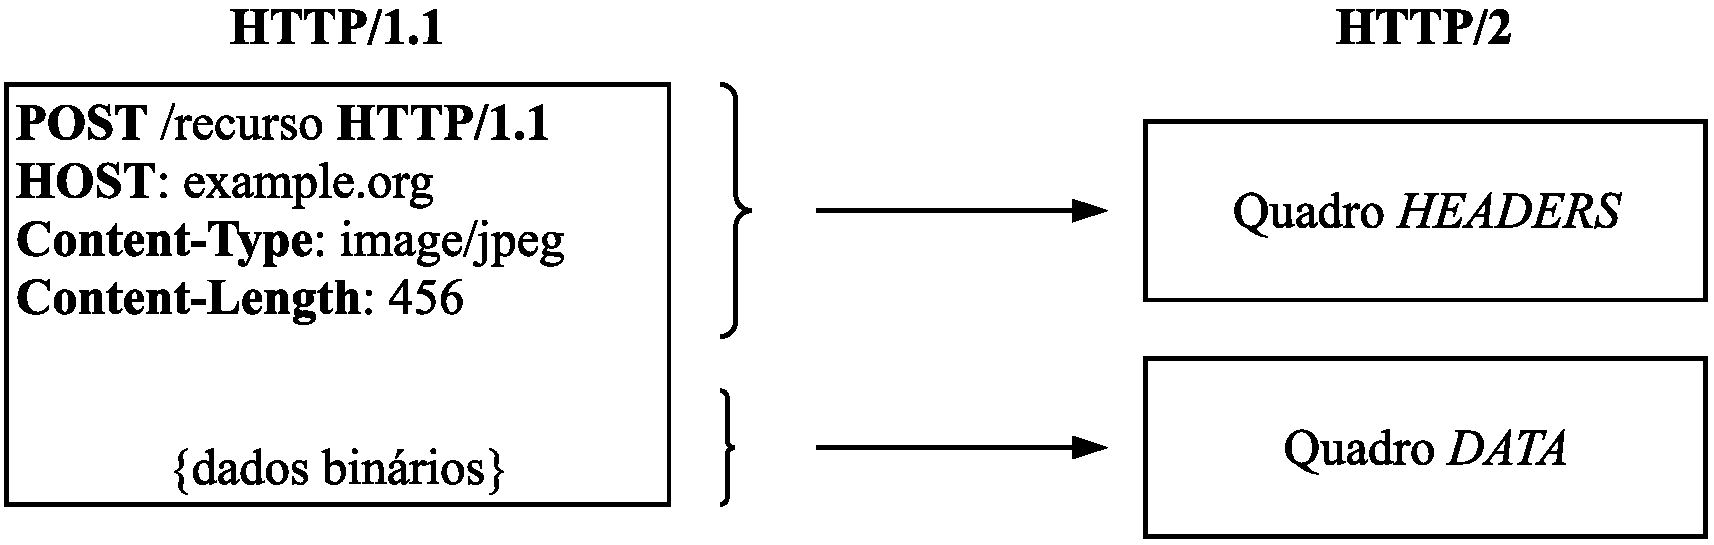
\includegraphics[width=\textwidth]{./fig/framing}
 \caption{Uma mensagem de requisição POST HTTP/1.1 e uma mensagem de requisição POST HTTP/2 equivalente.}
 \label{fig:framing}
\end{figure}

A especificação do HTTP/2 define um quadro como sendo a menor unidade de comunicação entre clientes e servidores. Um ou mais quadros podem ser enviados e recebidos tanto por clientes quanto servidores assim que o cliente inicia uma conexão TCP. Cada quadro é composto por um cabeçalho de tamanho fixo de 9 bytes seguido por um corpo de tamanho variado que depende do tipo do quadro.

\begin{figure}[hbt!]
 \centering
  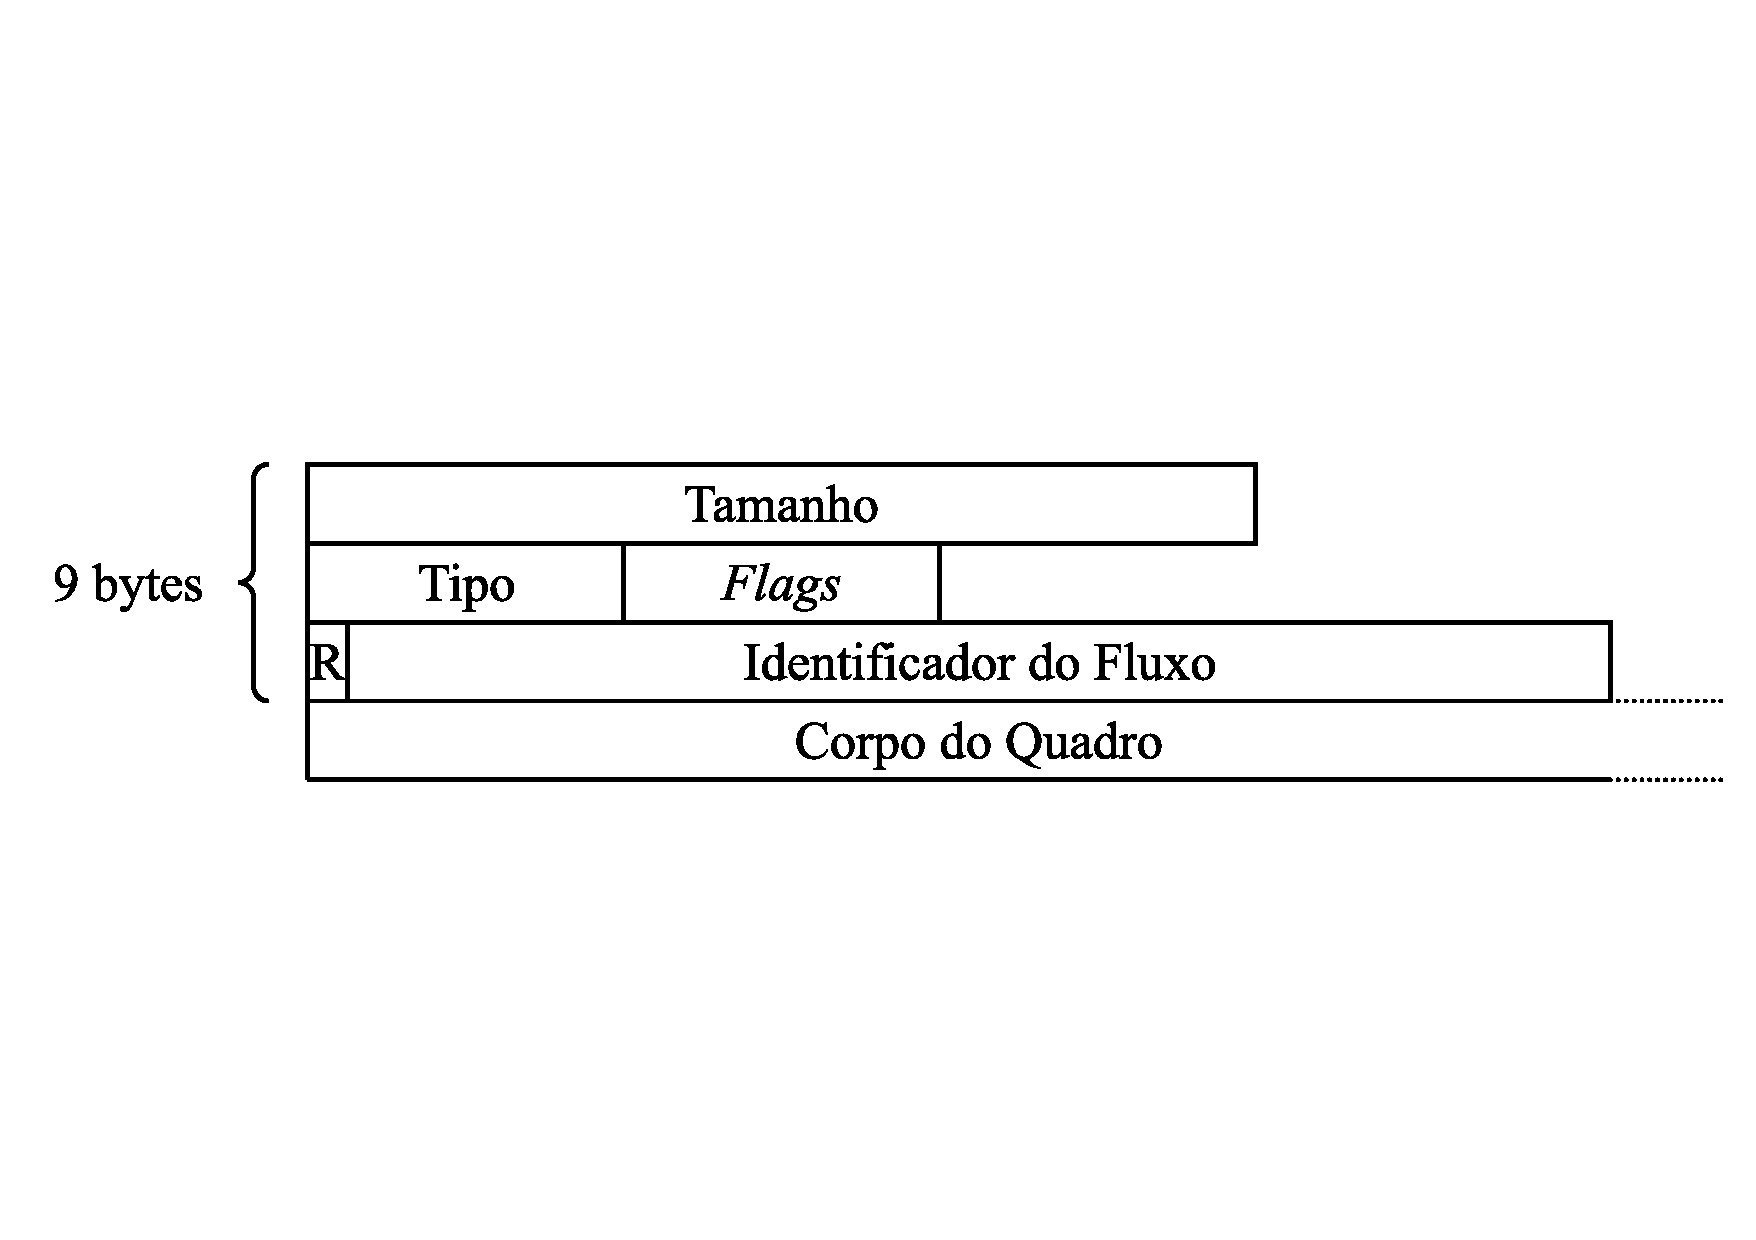
\includegraphics[width=\textwidth]{./fig/quadro}
 \caption{Formato de um quadro HTTP/2.}
 \label{fig:quadro}
\end{figure}

O formato de um quadro é mostrado na Figura \ref{fig:quadro}. O campo referente ao corpo do quadro varia em estrutura e conteúdo conforme o tipo do quadro. Os campos do cabeçalho do quadro são definidos como:

\begin{itemize}
    \item Tamanho (24 bits): carrega o tamanho do corpo do quadro (até $2^{24} - 1$ bytes).
    \item Tipo (8 bits): determina a estrutura e o conteúdo do corpo do quadro.
    \item {\em Flags} (8 bits): valor de 8 bits com significado específico para o tipo do quadro.
    \item R (1 bit): campo reservado que sempre possui valor 0.
    \item Identificador do Fluxo (31 bits): identifica unicamente um fluxo (ver Seção \ref{subsec:fluxos}).
\end{itemize}

Os seguintes tipos de quadros são definidos, cada um possuindo um papel distinto na comunicação HTTP/2:

\begin{itemize}
    \item {\em DATA}: transporta dados do corpo da mensagem.
    \item {\em HEADERS}: transporta campos de cabeçalhos da mensagem.
    \item {\em PRIORITY}: especifica a prioridade de um fluxo.
    \item {\em RST\_STREAM}: permite o fechamento de um fluxo.
    \item {\em SETTINGS}: transporta características de clientes e servidores para a conexão.
    \item {\em PUSH\_PROMISE}: sinaliza uma promessa para servir o recurso referenciado.
    \item {\em PING}: mede o RTT e verifica se uma conexão ociosa pode ser usada.
    \item {\em GOAWAY}: sinaliza o fechamento da conexão ou erros críticos.
    \item {\em WINDOW\_UPDATE}: permite implementação de controle de fluxo.
    \item {\em CONTINUATION}: continua uma sequência de campos de cabeçalhos.
\end{itemize}

\subsection{Fluxos de Mensagens}
\label{subsec:fluxos}

Um fluxo é definido como uma sequência independente e bidirecional de quadros dentro de uma conexão TCP e é identificado por um valor inteiro de 31 bits sem sinal. Tanto o cliente quanto o servidor podem criar e fechar um fluxo unilateralmente ou compartilhadamente entre si. Porém, clientes devem sempre criar um novo fluxo com valor {\em ímpar} maior que o valor do fluxo mais recentemente criado e servidores devem sempre criar um novo fluxo com valor {\em par} maior que o valor do fluxo mais recentemente criado. O fluxo de identificador 0 é reservado para controlar a conexão e não pode ser usado.

Clientes e servidores processam quadros de um fluxo na ordem em que são recebidos dentro da conexão TCP, podendo intercalar quadros de múltiplos fluxos concorrentemente abertos. Dessa forma, clientes e servidores são permitidos realizarem multiplexação de requisições e respostas associando cada troca de mensagens com um único fluxo.

Partindo do conhecimento da estrutura de um quadro, um fluxo pode ser examinado para que diferentes tipos de quadros sejam identificados, cada um com diferentes tamanhos. Como o tamanho é conhecido, o próximo quadro do fluxo pode ser processado mais eficientemente. Ao processar o cabeçalho do quadro, o seu corpo pode ser facilmente interpretado com base no seu tipo. Com isso, mensagens HTTP/2 são mais eficientes de serem processadas e mais compactas em transporte porque são binárias; mais robustas porque são menos propensas a erros; e mais simples porque existe apenas uma forma de processar uma mensagem.

\subsubsection{Ciclo de vida de um fluxo}

O ciclo de vida de um fluxo é exibido no diagrama da Figura \ref{fig:ciclo_fluxo}. As transições causam a mudança de um estado para outro de acordo com os quadros e {\em flags} enviados ou recebidos por clientes e servidores. Pressupõe-se que essas transições sejam geradas apenas pelo envio ou recebimento de quadros e {\em flags} ilustrados no diagrama. Por exemplo, não ocorre uma transição de estados quando quadros do tipo {\em CONTINUATION} seguem os quadros {\em HEADERS} ou {\em PUSH\_PROMISE} ou quando quadros do tipo {\em DATA} são enviados no estado aberto. Os estados são definidos como se segue:

\begin{itemize}
    \item ocioso: estado inicial de um fluxo.
    \item reservado (local): um cliente ou servidor {\em local} reservou um fluxo ocioso enviando um quadro do tipo {\em PUSH\_PROMISE}. 
    \item reservado (remoto): um cliente ou servidor {\em remoto} reservou um fluxo ocioso enviando um quadro do tipo {\em PUSH\_PROMISE}.
    \item aberto: estado onde clientes e servidores podem enviar quadros de qualquer tipo.
    \item semifechado (local): estado onde apenas quadros {\em WINDOW\_UPDATE}, {\em RST\_STREAM} e {\em PRIORITY} podem ser {\em enviados}, porém qualquer quadro pode ser {\em recebido}.
    \item semifechado (remoto): estado onde apenas quadros {\em WINDOW\_UPDATE}, {\em RST\_STREAM} e {\em PRIORITY} podem ser {\em recebidos}, porém qualquer quadro pode ser {\em enviado}. 
    \item fechado: indica o estado terminal de um fluxo, permitindo apenas o envio de quadros {\em PRIORITY}.
\end{itemize}

\begin{figure}[hbt!]
 \centering
  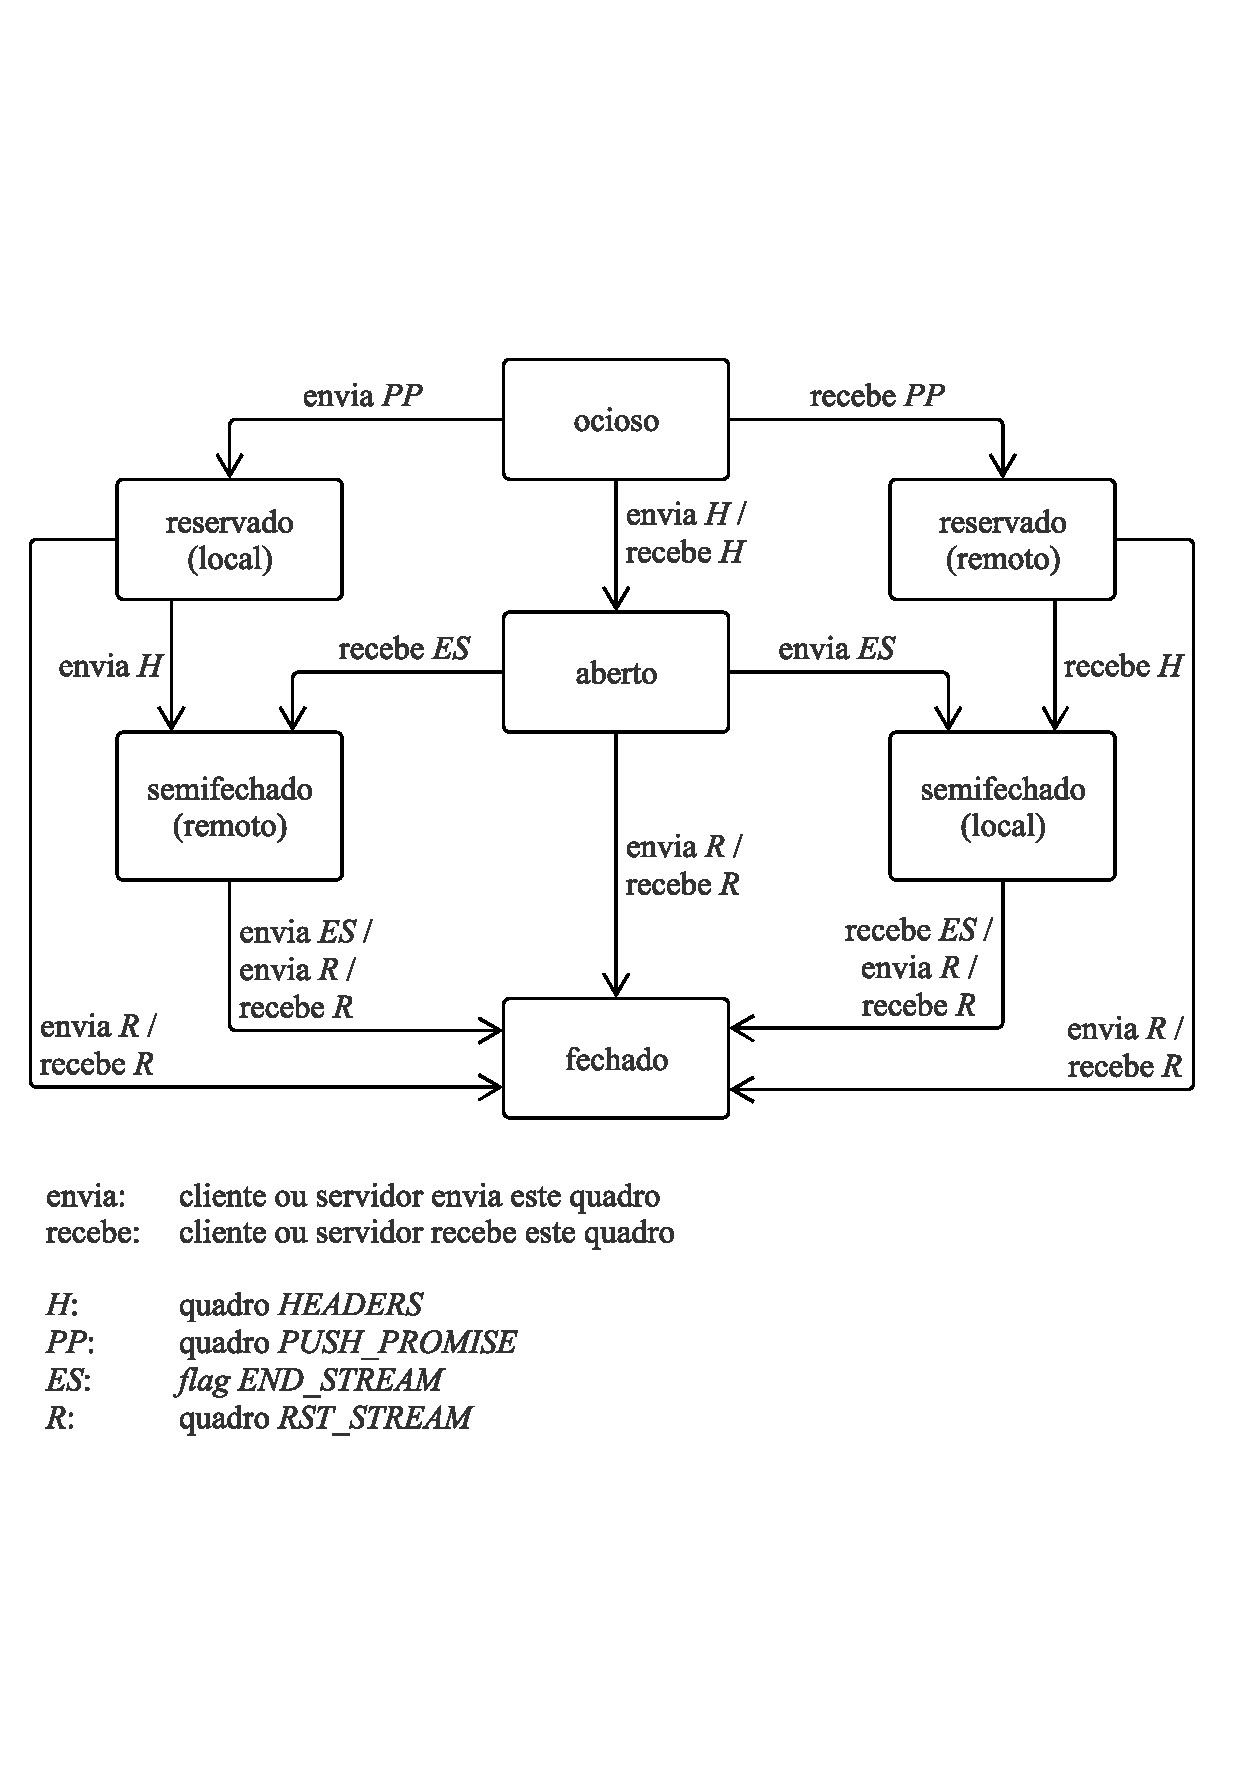
\includegraphics[width=\textwidth]{./fig/ciclo_fluxo}
 \caption{O ciclo de vida de um fluxo HTTP/2 ilustrado através de um diagrama com transição de estados.}
 \label{fig:ciclo_fluxo}
\end{figure}

\subsubsection{Controle de fluxo}

Se vários fluxos multiplexados (que carregam mensagens de requisição\slash resposta) estão sendo enviados pela conexão TCP, mas apenas um deles está entregando quadros, ele bloqueia outros fluxos. Visando resolver esse problema, um controle de fluxo é necessário para impedir que um fluxo interfira com outros fluxos, permitindo usá-los de modo mais eficiente. Para isso, a especificação do HTTP/2 define sete princípios de controle de fluxo, tais quais foram extraídos e traduzidos diretamente do documento RFC 7540 \cite{BelsheRFC7540}:

\begin{enumerate}
    \item O controle de fluxo é específico para uma conexão. Os dois tipos de controle de fluxo acontecem entre clientes e servidores em um único salto e não em todo o caminho de fim a fim.
    \item O controle de fluxo é implementado com o uso de quadros {\em WINDOW\_UPDATE} e é baseado em um esquema de créditos, já que cada destinatário (cliente ou servidor que está recebendo quadros) anuncia sua janela inicial (em bytes) que ele está preparado para receber em um fluxo e para toda a conexão. Essa janela é reduzida sempre que um remetente envia um quadro do tipo {\em DATA} e incrementado via quadros {\em WINDOW\_UPDATE} enviados pelo destinatário.
    \item O controle de fluxo é direcional com o controle geral fornecido pelo destinatário. Um destinatário pode optar por definir qualquer tamanho de janela que desejar para cada fluxo e para toda a conexão. Um remetente deve respeitar os limites de controle de fluxo impostos por um destinatário. Clientes, servidores e intermediários anunciam, independentemente, sua janela de controle de fluxo como um destinatário e cumprem os limites de controle de fluxo definidos por destinatários quando estiverem atuando como remetentes.
    \item O valor inicial da janela de controle de fluxo é de 65.535 bytes tanto para novos fluxos quanto para a conexão em geral.
    \item O tipo de quadro determina se o controle de fluxo se aplica a um quadro. Somente os quadros do tipo {\em DATA} estão sujeitos ao controle de fluxo; todos os outros tipos de quadro não consomem espaço na janela de controle de fluxo anunciada. Isso garante que estruturas de controle importantes não sejam bloqueadas pelo controle de fluxo.
    \item O controle de fluxo não pode ser desativado.
    \item O HTTP/2 define apenas o formato e a semântica do quadro {\em WINDOW\_UPDATE}. A especificação não estipula como um destinatário decide quando enviar esse quadro ou o valor que ele envia, nem como um remetente escolhe enviar pacotes. As implementações são capazes de selecionar qualquer algoritmo que atenda às suas necessidades.
\end{enumerate}

Ainda de acordo com a especificação, as implementações também são responsáveis por gerenciar como as requisições e as respostas são enviadas com base na prioridade, escolhendo como evitar o bloqueio de requisições e gerenciar a criação de novos fluxos. As escolhas de algoritmo para estas poderiam interagir com qualquer algoritmo de controle de fluxo. Os remetentes sempre estão sujeitos a respeitar a janela de controle de fluxo anunciada pelo destinatário, mas destinatários que não desejarem controle de fluxo podem anunciar uma janela de tamanho máximo ($2^{31} - 1$) e podem manter essa janela enviando um quadro {\em WINDOW\_UPDATE} quando qualquer quadro {\em DATA} é recebido.

\subsection{HPACK: Compressão de Cabeçalhos}
\label{subsec:compression}

Para toda requisição\slash resposta do HTTP/1.1, os mesmos cabeçalhos extensos e redundantes são enviados e recebidos durante uma conexão TCP. Isso resulta em problemas de congestionamento de rede. Para resolver isso, um padrão de compressão de cabeçalhos HTTP/2 para um formato binário foi aprovado pela IETF, denominado HPACK \cite{BelsheRFC7541}.

A especificação do HTTP/2 define listas de cabeçalhos como zero ou mais campos de cabeçalhos. Campos de cabeçalhos são os tradicionais nomes com um ou mais valores associados. Essas listas são serializadas em um bloco de cabeçalhos utilizando os algoritmos definidos em HPACK. Esse bloco de cabeçalhos é então dividido em uma ou mais cadeias de bytes e carregadas no corpo de quadros {\em HEADERS}, {\em PUSH\_PROMISE} ou {\em CONTINUATION}. Um cliente ou um servidor que está recebendo esses cadeias de bytes os concatenam e depois descomprimem o bloco para reconstruir a lista decodificada.  Os principais elementos do HPACK são os seguintes \cite{Yamamoto:2017:EHH:3095786.3095787}:

\begin{itemize}
    \item Campo de cabeçalhos.
    \item Bloco de cabeçalhos.
    \item Tabela estática.
    \item Tabela dinâmica.
    \item Codificador.
    \item Decodificador.
\end{itemize}

Um campo de cabeçalho é um par (nome, valor), que são uma sequência de bytes. Campos de cabeçalhos codificados são representados ou como um valor numérico (índice) ou como um valor literal. Na representação de índice, existe uma referência para uma entrada na tabela estática ou na tabela dinâmica. Na representação literal, existe um par (nome, valor) onde um nome ou é representado literalmente ou é uma referência para uma entrada na tabela estática ou na tabela dinâmica e um valor é representado literalmente.

Um bloco de cabeçalho é uma concatenação de representações de campos de cabeçalhos descritos no parágrafo anterior. Um decodificador pode processar um bloco de cabeçalho sequencialmente para reconstruir a lista de cabeçalhos original.

Uma tabela estática é uma estrutura de dados do tipo lista e é predefinida em \cite{BelsheRFC7541} com uma lista estática de campos de cabeçalhos, podendo ser referenciada por um índice cujos valores são pares (nome do cabeçalho, valor do cabeçalho). Por exemplo, o índice 2 possui o par (``:method'', ``GET'') e o índice 19 possui o par (``accept'', `'), sem valor do cabeçalho. A tabela estática associa estaticamente campos de cabeçalhos que ocorrem frequentemente para índices. Trata-se de uma tabela ordenada, de apenas leitura ({\em read-only}), é sempre acessível e compartilhada em todos os contextos de codificação e decodificação.

Uma tabela dinâmica é uma estrutura de dados similar à tabela estática, com a diferença de que as entradas são criadas dinamicamente. Ela tem um limite superior ao seu tamanho e se a criaçao de novas entradas ultrapassar esse tamanho, as entradas mais antigas são removidas. Clientes e servidores mantêm uma tabela dinâmica para o envio e outra para o recebimento de campos de cabeçalhos (correspondem a contextos de codificação e decodificação, respectivamente). Elas operam seguindo o princípio FIFO ({\em First In, First Out}) e associam campos de cabeçalhos para índices e é específica para um contexto de codificação\slash decodificação. As tabelas dinâmicas podem ser usadas pelo codificador para indexar campos de cabeçalhos redundantes e é permitido que ela contenha entradas duplicadas.

O codificador é implementado com o auxílio das tabelas estáticas e dinâmicas que mapeiam campos de cabeçalhos para índices. Sua função é atualizar a tabela dinâmica e ordenar os campos de cabeçalho no bloco de cabeçalho de acordo com a ordem original da lista de cabeçalho. Na verdade, existem três métodos de compressão utilizados pelo codificador para codificar campos de cabeçalhos: tabelas estáticas, tabelas dinâmicas e código de Huffman estático. Já o decodificador compartilha as modificações prescritas pelo codificador e mantém uma tabela dinâmica como um contexto de decodificação para descomprimir blocos de cabeçalhos.

\subsection{Priorização de Requisições}
\label{subsec:priority}

Priorizar uma requisição é permitir que clientes informem a quantidade de recursos (como CPU, memória e taxas de transmissão de dados) que devem ser alocados a essa requisição em relação a outras requisições. Visto que vários fluxos carregando requisições podem estar concorrentemente abertos em uma comunicação HTTP/2, clientes podem atribuir informações de priorização para um fluxo específico quando ele é aberto (enviando um quadro do tipo {\em HEADERS}) e em qualquer momento da comunicação essa prioridade pode ser alterada enviando um quadro do tipo {\em PRIORITY}.

Para isso, o HTTP/2 permite que dependências por um fluxo sejam associados a um outro fluxo que depende do seu término. Caso dois ou mais fluxos sejam dependentes do término do mesmo fluxo, um peso (um número inteiro entre 1 e 256) pode ser atribuído para cada fluxo dependente para informar que os recursos disponíveis devem ser alocados em proporção aos seus pesos.

O mecanismo de dependências e pesos de fluxos para permitir priorização pode ser ilustrado através de uma árvore de dependências. Por exemplo, considere a árvore de dependências da Figura \ref{fig:dependency_tree}. Cada nó representa um fluxo, sendo que o número fora dos parênteses é o seu identificador e o número dentro dos parênteses é o seu peso.

\begin{figure}[hbt!]
 \centering
  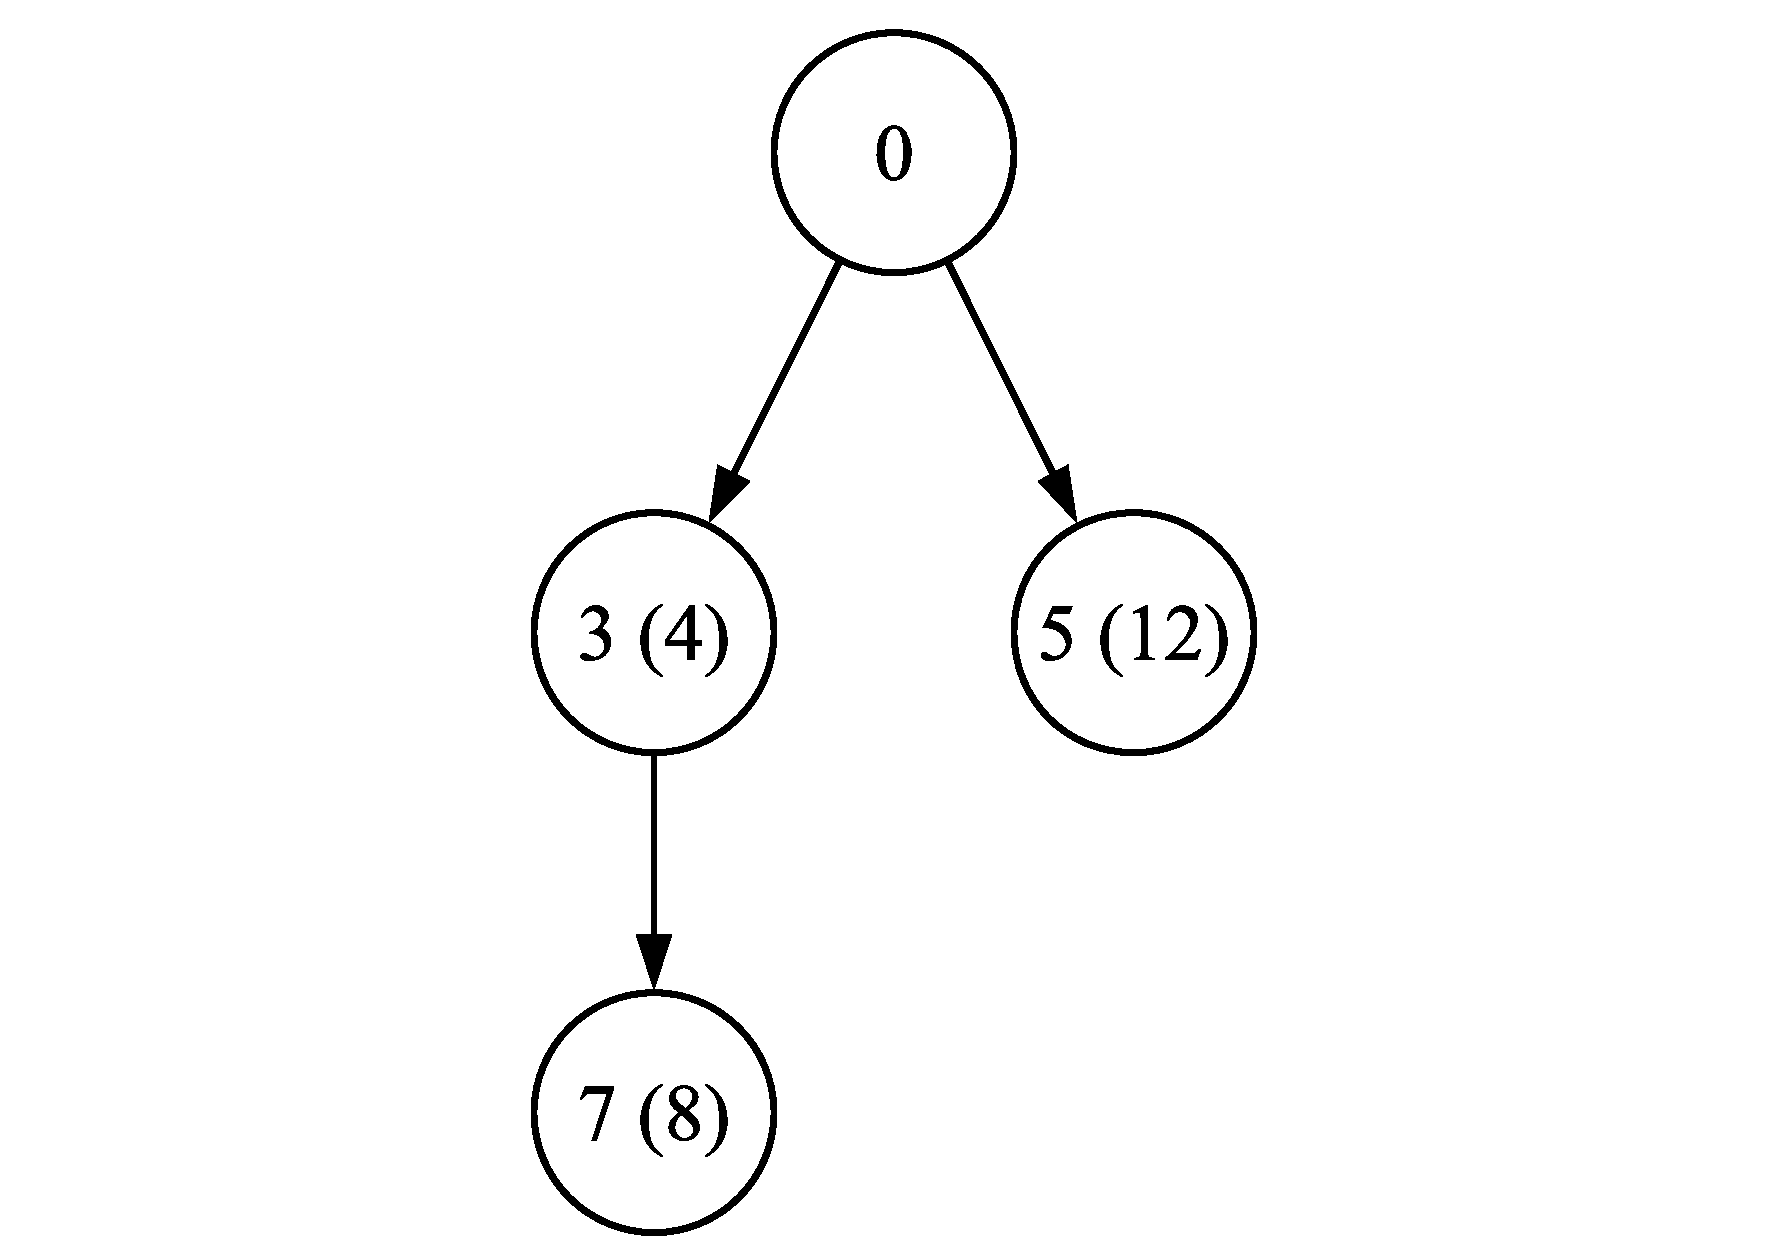
\includegraphics[width=0.5\textwidth]{./fig/dependency_tree}
 \caption{Dependências e pesos de fluxos HTTP/2 como uma árvore de dependências.}
 \label{fig:dependency_tree}
\end{figure}

Todo fluxo que não tem dependência declarada depende do fluxo 0 (conforme visto na subseção \ref{subsec:fluxos}, um fluxo de valor 0 é reservado para a conexão), que forma a raiz da árvore. Sendo assim, os fluxos 3 e 5 dependem do fluxo 0 e o fluxo 7 depende do fluxo 3. Como os fluxos 3 e 5 são dependentes do mesmo fluxo, a alocação de recursos é distribuída proporcionalmente em relação aos seus pesos: o fluxo 3 recebe 1/4 (4/16) e o fluxo 5 recebe 3/4 (12/16) dos recursos disponíveis.

\subsection{{\em Push} de Requisição\slash Resposta do Servidor}
\label{subsec:push}

Uma página Web típica inclui vários recursos independentes e que precisam ser requisitados separadamente por um cliente HTTP. Por exemplo, o arquivo HTML padrão de um servidor (comumente referido como {\em index.html}) pode incluir recursos dinâmicos como arquivos JavaScript, CSS e imagens que são necessários para exibir a página corretamente. No HTTP, o cliente precisa requisitar cada um desses recursos separadamente.

No HTTP/2, um servidor pode enviar várias respostas para uma única requisição de um cliente, ou seja, um servidor pode fazer um {\em push} (forçar) o envio de duas ou mais respostas contendo recursos associados a requisição original por um recurso, sem que clientes tenham que requisitar cada recurso separadamente. Assim, o servidor pode enviar antecipadamente todos os recursos dinâmicos contidos em uma página, sem que o cliente precise requisitar cada um.

O {\em push} do servidor é dividido em {\em push} de requisição e {\em push} de resposta. No {\em push} de requisição, o servidor envia um quadro do tipo {\em PUSH\_PROMISE} junto com campos de cabeçalhos (assim como nos cabeçalhos de uma requisição normal de um cliente) no estado ocioso de um fluxo, indicando que esse fluxo será reservado para um futuro {\em push} de resposta. Depois de enviado esse quadro, o servidor começa a enviar respostas assim que uma requisição tenha sido explicitamente feita pelo cliente.

É importante observar que o cliente pode desabilitar o {\em push} do servidor e que, por medidas de segurança, o servidor precisa ser autoritativo pelas respostas enviadas. O cliente também pode optar por recusar um {\em push} do servidor enviando um quadro do tipo {\em RST\_STREAM}. Assim, o cliente tem completo controle sobre como o {\em push} do servidor é usado.

\section{Lua}
\label{sec:lua}

A linguagem de programação Lua \cite{Ierusalimschy:2009:PMP:2175094.2175096, Ierusalimschy2016PiL, Ierusalimschy2018:LDL:3289258.3186277}  foi criada no início dos anos 1990 por Roberto Ierusalimschy, Waldemar Celes e Luis Henrique de Figueiredo na Pontifícia Universidade Católica do Rio de Janeiro (PUC-Rio). É uma linguagem de {\em scripting} multiparadigma que oferece suporte principalmente ao paradigma de programação procedural, embora também seja usada em programação concorrente, programação orientada a objetos, programação funcional, entre outros paradigmas. Lua também oferece suporte à descrição de dados, no estilo de JSON ou XML.

Atualmente, Lua é utilizada em várias aplicações industriais, com uma ênfase em sistemas embarcados e jogos, sendo a linguagem de {\em scripting} mais utilizada em jogos do mundo. Ela também é considerada uma das linguagens de {\em scripting} de melhor desempenho do mundo, devido a sua implementação eficiente.

Lua tem tipagem dinâmica, estruturas de dados dinâmicas, gerenciamento automático de memória e outras construções de linguagem similares às de outras linguagens de {\em scripting} dinamicamente tipadas. O que separa Lua unicamente dessas linguagens é o seu projeto, que foi definido em função dos seguintes objetivos:

\begin{itemize}
    \item Extensibilidade: Lua é uma biblioteca escrita em C e possui uma API C usada tanto para ser estendida com novas características quanto para estender outras aplicações escritas em C. De fato, a extensibilidade impactou fortemente o projeto de Lua \cite{Ierusalimschy2011passing}.
    \item Simplicidade: Lua é uma linguagem simples e pequena. Ao invés de ter incontáveis construções de linguagem feitas para resolver um determinado problema, Lua possui poucos (mas flexíveis) conceitos que atendem diferences necessidades.
    \item Eficiência: A implementação de Lua é pequena em tamanho. Isso a torna uma implementação muito eficiente e portátil. Como Lua é leve e eficiente, uma aplicação que embute Lua não é sobrecarregada.
    \item Portabilidade: Lua pode ser executada em praticamente todas as plataformas existentes por ser escrita em ANSI (ISO) C. Por ser pequena, Lua executa facilmente nessas plataformas sem que elas sejam negativamente impactadas.
\end{itemize}

\subsection{Tabelas e Funções}
\label{subsec:tables}

Lua é bastante reconhecida por sua simplicidade em harmonia com sua flexibilidade de programação. Muitas construções da linguagem são criadas a partir de duas construções mais básicas: tabelas e funções. Ambas construções permeiam toda a linguagem e formam a base para mecanismos mais complexos como módulos e programação orientada a objetos.

A tabela é uma estrutura de dados dinâmica e constitui a única estrutura de dados de Lua. As tabelas de Lua são semelhantes aos vetores associativos de Perl e PHP, que são compostas por pares (chave, valor). É fácil pensar em uma tabela como um {\em map} ou como uma tabela {\em hash} por associarem uma chave a um valor. Tabelas são usadas para implementar as mais diversas estruturas de dados (tais como vetores, registros, listas, filas, pilhas e conjuntos) de modo eficiente e são as construções que permitem criar outras construções mais complexas da linguagem. Logo, tabelas permeiam toda a linguagem Lua.

Lua suporta diferentes mecanismos para construir tabelas. A expressão \verb|t["x"] = 1| cria uma tabela \verb|t| onde a chave \verb|"x"| é associada ao valor 1 e a expressão \verb|t[1] = "x"| cria uma tabela \verb|t| associando a chave 1 ao valor \verb|"x"|. Utilizando o chamado ``açúcar sintático'' de Lua, a primeira expressão pode ser escrita como \verb|t.x = 1|. Utilizando a sintaxe de construtor \verb|{}|, o construtor \verb|{x = 1, y = 2}| cria uma tabela com duas entradas, uma associando \verb|"x"| ao valor 1 e outra associando \verb|"y"| ao valor 2 \cite{Ierusalimschy2018:LDL:3289258.3186277}.

As funções de Lua têm funcionalidades tradicionais às de outras linguagens de programação, mas com o diferencial de que elas são valores de primeira classe, isto é, uma função pode ser armazenada em variáveis, passada como argumento para parâmetros de outras funções e ser retornada como resultado dessas outras funções. Lua também oferece suporte a funções com escopo léxico ({\em closures}), habilitando Lua a ser utilizada para programação funcional. O código abaixo mostra uma função anônima sendo atribuída a variável \verb|mod|:

\begin{Verbatim}
mod = function(x, y)
  return x % y
end
\end{Verbatim}

Tabelas e funções de primeira classe podem ser usados para implementar módulos em Lua (semelhantes a pacotes em Java e Perl, ou {\em namespaces} em C++), que servem como bibliotecas ou como um espaço de nomes para a linguagem. Por exemplo, considere o Código \ref{code:ponto}, que mostra como uma biblioteca simples em Lua que permite criar pontos (coordenadas) e calcular a distância entre dois pontos pode ser criada. Um programador pode (re)usar essa biblioteca usando a função \verb|require| da biblioteca padrão (Código \ref{code:test_ponto}).

\begin{center}
 \begin{minipage}{0.7\textwidth}
  \begin{codigo}[H]
   \small
   \VerbatimInput[xleftmargin=10mm,numbers=left,obeytabs=true]{./prog/ponto.lua}
   \caption{\texttt{Biblioteca "ponto"}}
   \label{code:ponto}
  \end{codigo}
 \end{minipage}
\end{center}

\begin{center}
 \begin{minipage}{0.7\textwidth}
  \begin{codigo}[H]
   \small
   \VerbatimInput[xleftmargin=10mm,numbers=left,obeytabs=true]{./prog/test_ponto.lua}
   \caption{\texttt{Utilizando a biblioteca "ponto"}}
   \label{code:test_ponto}
  \end{codigo}
 \end{minipage}
\end{center}

A função \verb|require| mostrada na linha 1 do Código \ref{code:test_ponto} é um exemplo de uma das funções fornecidas pela biblioteca padrão de Lua. Além dessa função, a função \verb|math.sqrt| é exibida na linha 10 do Código \ref{code:ponto}, que faz parte da biblioteca padrão \verb|math| de Lua. A biblioteca ``ponto'' é um exemplo de uma biblioteca externa que pode ser criada por programadores Lua como forma de estender as funcionalidades da linguagem. Elas não vêm inclusas no conjunto de bibliotecas padrões de Lua e devem ser incluídas manualmente no código caso o programador deseje usá-la.

Tabelas e funções também podem ser utilizadas para simular programação orientada a objetos. Conceitos de orientação a objetos como classes, objetos, métodos e herança podem ser representados por tabelas e funções, seguindo o padrão de utilizar mecanismos básicos da linguagem para construir mecanismos mais complexos.

Por exemplo, considere o Código \ref{code:class}, onde uma classe nomeada {\em class} é implementada em Lua. Essa classe faz o uso de dois métodos: \verb|set_value(value)| define um novo valor \verb|value| e \verb|get_value()| recupera esse valor. Um construtor \verb|new| também é definido para instanciar objetos dessa classe. Lua possibilita a criação de classes com o auxílio da função \verb|setmetatable| para instanciar tabelas a partir de outras tabelas e do metamétodo \verb|__index| para acessar valores dessas tabelas. Além disso, Lua provê o ``açúcar sintático'' de dois-pontos para criar um parâmetro de autoreferência (normalmente chamado de {\em this} ou {\em self} em outras linguagens de programação orientadas a objetos).

O Código \ref{code:object} mostra como um objeto pode ser instanciado a partir de uma classe (representada por um módulo). Na linha 3, o código cria um novo objeto a partir da classe \verb|class| utilizando seu construtor \verb|new|, configura o valor 2 para esse objeto e depois recupera esse mesmo valor chamando os métodos da classe \verb|class|.

\begin{center}
 \begin{minipage}{0.7\textwidth}
  \begin{codigo}[H]
   \small
   \VerbatimInput[xleftmargin=10mm,numbers=left,obeytabs=true]{./prog/class.lua}
   \caption{\texttt{Classe}}
   \label{code:class}
  \end{codigo}
 \end{minipage}
\end{center}

\begin{center}
 \begin{minipage}{0.7\textwidth}
  \begin{codigo}[H]
   \small
   \VerbatimInput[xleftmargin=10mm,numbers=left,obeytabs=true]{./prog/object.lua}
   \caption{\texttt{Objeto}}
   \label{code:object}
  \end{codigo}
 \end{minipage}
\end{center}

\subsection{Co-rotinas}
\label{subsec:coroutines}

O suporte à programação concorrente em Lua é fornecido por co-rotinas e funcionam como {\em multithreading} cooperativa: apenas uma co-rotina ({\em thread}) está em execução por vez, e a troca de contexto entre as co-rotinas é feita de forma explícita. Diferentemente de {\em multithreading} preemptiva, onde a troca de contexto entre as {\em threads} ocorre de forma implícita, na cooperativa existem funções explícitas para a transferência de controle.

Co-rotinas são, assim como funções, valores de primeira classe. Outra característica de co-rotinas em Lua é que elas são assimétricas, ou seja, existe uma função para suspender uma co-rotina e outra função para executar uma co-rotina. Isso as distingue de co-rotinas simétricas, onde apenas uma função exerce esse papel.

Uma co-rotina é criada através da biblioteca padrão \verb|coroutine| de Lua. Assim como a biblioteca padrão \verb|table| de Lua, a biblioteca \verb|coroutine| é um módulo nativo da linguagem Lua, consistindo de tabelas e funções. As principais funções que fazem parte do módulo \verb|coroutine| são:

\begin{itemize}
    \item \verb|coroutine.create|: cria uma co-rotina.
    \item \verb|coroutine.yield|: suspende uma co-rotina.
    \item \verb|coroutine.resume|: coloca uma co-rotina em execução.
    \item \verb|coroutine.status|: verifica o estado de uma co-rotina.
\end{itemize}

O funcionamento de uma co-rotina pode ser ilustrado através de um exemplo de código. No Código \ref{code:coroutine}, que foi adaptado de \cite{Ierusalimschy2018:LDL:3289258.3186277}, uma co-rotina é criada na linha 1 pela função \verb|coroutine.create|, passando uma função anônima como seu parâmetro. Essa função apenas cria a co-rotina, sem executá-la. Na linha 2, o valor de \verb|x| passado como parâmetro será 1 porque a função \verb|coroutine.resume| na linha 8 passou esse valor como argumento. Na linha 3, a co-rotina suspende a execução, passando o valor 2 como argumento de \verb|coroutine.yield| para \verb|coroutine.resume| na linha 8 e armazenando esse valor na variável \verb|y|. Depois, o programa retorna a executar a co-rotina, dessa vez passando o valor 3 como argumento de \verb|coroutine.resume| na linha 9 para o retorno de \verb|coroutine.yield| na linha 3. Por fim, a co-rotina causa o término de \verb|coroutine.resume| na linha 9 retornando o valor 4 e armazenando-o na variável \verb|y|.

\begin{center}
 \begin{minipage}{0.7\textwidth}
  \begin{codigo}[H]
   \small
   \VerbatimInput[xleftmargin=10mm,numbers=left,obeytabs=true]{./prog/coroutine.lua}
   \caption{\texttt{Co-rotina}}
   \label{code:coroutine}
  \end{codigo}
 \end{minipage}
\end{center}

Uma desvantagem em utilizar co-rotinas é que gerenciá-las pode se tornar uma tarefa complexa quando o número de suspensões e retomadas aumentam. Por exemplo, se uma co-rotina invoca uma operação bloqueantes de rede como \verb|receive| e bloqueia, todo o programa é bloqueado até que a operação termine. Esse comportamento pode ser evitado fornecendo um conjunto de funções não bloqueantes que iniciam uma operação de rede e suspende a co-rotina ativa quando a operação não puder ser imediatamente completada.

Ierusalismchy \cite{Ierusalimschy2016PiL} mostra um exemplo de uma aplicação concorrente que utiliza co-rotinas com funções não bloqueantes da API {\em socket} do LuaSocket \cite{Nehab2007}. Uma outra forma de evitar esse comportamento indesejável em aplicações concorrentes é criando um escalonador de co-rotinas, que gerencia a tarefa de suspender e executar co-rotinas quando as operações de rede bloquearem. Uma biblioteca em Lua que proporciona essa funcionalidade é chamada Copas, descrita na seção a seguir.

\subsection{Copas}
\label{subsec:copas}

Copas ({\em Coroutine Oriented Portable Asynchronous Services for Lua}) \cite{Copas} é uma biblioteca que oferece suporte a operações assíncronas para aplicações de rede escritas em Lua e seu foco é na criação de clientes e servidores. Funções assíncronas são fornecidas pela biblioteca Copas para impedir que a aplicação de rede fique bloqueada em uma chamada de rede tipicamente bloqueante (por exemplo, na função de recebimento de dados \verb|receive|). Para isso, Copas faz uso da característica de {\em multithreading} cooperativa de Lua, atuando como um escalonador de co-rotinas.

Copas utiliza a biblioteca LuaSocket \cite{Nehab2007} para interagir com sua API {\em socket}. Com funcionamento semelhante às funções \verb|socket.send| e \verb|socket.receive| do LuaSocket, a função \verb|copas.send| envia dados pelo {\em socket} e a função \verb|copas.receive| recebe dados pelo {\em socket}. A diferença entre essas funções em ambas as bibliotecas é que em Copas não existem chamadas bloqueantes. O uso de {\em multithreading} cooperativa de Lua permite que os envios e recebimentos de dados pelo {\em socket} sejam tratados de forma simultânea em várias {\em threads}, desde que elas façam chamadas às funções \verb|copas.send| e \verb|copas.receive| de Copas.

A tarefa de escalonar co-rotinas é realizada pelo escalonador do Copas, onde um {\em loop} principal fica responsável principalmente por empregar um mecanismo de consulta para verificar se o resultado da computação de uma função não bloqueante de um {\em socket} (por exemplo, recebimento de dados ou {\em time out}) já está disponível. Quando o resultado é recebido, o escalonador utiliza co-rotinas para processá-lo concorrentemente com outras co-rotinas contendo resultados de computação de outras funções não bloqueantes. Com isso, a execução assíncrona de uma aplicação de rede é alcançada, pois o uso de funções não bloqueantes de um {\em socket} em combinação com a facilidade de executá-las concorrentemente com várias {\em threads} nunca travam o {\em loop} principal da aplicação. As seguintes funções de Copas implementam esse gerenciamento de co-rotinas:

\begin{itemize}
    \item \verb|copas.loop|: inicia o {\em loop} principal do Copas.
    \item \verb|copas.addthread|: adiciona uma nova co-rotina ao escalonador para que ele possa escalonar essa co-rotina quando o resultado de uma computação assíncrona de rede for recebida.
    \item \verb|copas.sleep|: assim como a função \verb|coroutine.yield| vista na Subseção \ref{subsec:coroutines}, suspende a execução da co-rotina atual (apenas uma pode estar em execução) criada por \verb|copas.addthread|.
    \item \verb|copas.wakeup|: volta a executar a co-rotina criada por \verb|copas.addthread| e passada como parâmetro para essa função.
\end{itemize}

Para ilustrar um caso de uso do Copas, considere o Código \ref{code:repetidor}, que demonstra um simples uso de um repetidor que transmite de volta os dados recebidos e termina quando recebe \verb|quit|. Para simplificar, o código para criação do {\em socket} que utiliza a API do LuaSocket foi omitido. Primeiramente, nas linhas 19 e 20, as {\em threads} \verb|on_quit| e \verb|despachante| são adicionadas ao escalonador do Copas, respectivamente. A {\em thread} \verb|despachante| é simplesmente um {\em loop} que recebe dados provenientes de um {\em socket} e verifica se esses dados correspondem a \verb|quit|, sinalizando o término do envio de dados. A {\em thread} \verb|on_quit| é uma tratadora dessa sinalização de \verb|quit|, que é despachada quando os dados param de ser enviados.

Depois de adicionadas as {\em threads}, o {\em loop} principal do Copas começa a executar, na linha 22. A primeira {\em thread} que ele escalona é \verb|on_quit|, pois foi a primeira a ser adicionada. Em seguida, na linha 14, essa {\em thread} é colocada em modo suspenso porque ela só poderá ser despachada quando os dados pararem de serem enviados pelo {\em socket}, ou seja, quando \verb|quit| é recebido. Assim que a {\em thread} \verb|on_quit| é suspendida, a {\em thread} \verb|despachante| é escalonada pelo {\em loop} principal, que começa a verificar pela sinalização do término do envio de dados. Caso os dados ainda estejam sendo enviados pelo remetente, esses mesmos dados são enviados para o mesmo, repetindo o ciclo. Quando os dados correspondentes a \verb|quit| são recebidos, a {\em thread} \verb|on_quit| é despachada na linha 5 e o programa é finalizado, pois não há mais nenhuma co-rotina e nenhum {\em socket} a serem escalonados pelo {\em loop} do Copas.

\begin{center}
 \begin{minipage}{0.7\textwidth}
  \begin{codigo}[H]
   \small
   \VerbatimInput[xleftmargin=10mm,numbers=left,obeytabs=true]{./prog/repetidor.lua}
   \caption{\texttt{Repetidor Copas}}
   \label{code:repetidor}
  \end{codigo}
 \end{minipage}
\end{center}

\section{Trabalhos Relacionados}
\label{sec:relatedwork}

Muitos esforços vêm sendo realizados para implementar bibliotecas clientes HTTP/2. O principal problema enfrentado pelos trabalhos que se propõem a implementar bibliotecas do lado cliente do HTTP/2 é o de construir um escalonador de fluxos. A exigência do HTTP/2 é de que fluxos concorrentes devem ser processados fora de ordem, porém a ordem com que os quadros são transmitidos dentro desses fluxos é relevante \cite{BelsheRFC7540}. Por esses motivos, os trabalhos de implementação de bibliotecas clientes HTTP/2 necessitam intercalar quadros provenientes de múltiplos fluxos em ordem, finalizar o processamento de um fluxo e decidir qual será o próximo fluxo a ser processado. Assim, todos os trabalhos revisados neste estudo empregam o modelo de programação concorrente, apesar das diferentes construções de linguagens de programação envolvidas para realizá-lo.

Um segundo problema que as bibliotecas tentam resolver é o modo de implementar o ciclo de vida de um fluxo. Parece que existe um consenso de que o modelo de programação mais apropriado para representar esse ciclo é o de orientação a eventos. Esse modelo de fato traz vantagens sobre a estruturação tanto do código de API de alto nível quanto do código HTTP/2 de baixo nível, pois os estados e as transições do ciclo de vida de um fluxo podem ser programadas em máquinas de estados, um mecanismo muito semelhante à programação orientada a eventos. Nesse contexto, com exceção de uma biblioteca, todos os outros trabalhos revisados neste estudo empregam o modelo de programação orientada a eventos, apesar das diferentes construções de linguagens de programação envolvidas para realizá-la.

A biblioteca HTTP/2 atualmente em uso para Lua (lua-http) \cite{DaurminatorLuaHTTP} depende de uma biblioteca externa denominada cqueues para obter a facilidade de tratar {\em threads}, sinais e notificações para implementarem concorrência e eventos associados aos fluxos. Ela também faz uso extenso do {\em loop} principal de cqueues, que é modularizável e que pode ser facilmente controlado externamente. No entanto, o problema da biblioteca cqueues é que ela faz uso de primitivas ao nível do {\em kernel} do sistema operacional, o que impõe limitações de portabilidade na biblioteca lua-http. Como consequência, essa biblioteca apenas funciona em sistemas operacionais UNIX.

A biblioteca cliente HTTP/2 para Node.js (http2) \cite{Nodejs}, assim como lua-http, também é completa em termos das especificações de um cliente HTTP/2. Diferentemente de Lua, Node.js é uma tecnologia com um {\em loop} principal nativo embutido em todo código JavaScript que seja interpretado por Node.js. Essa característica o torna ideal para modelar a programação orientada a eventos e consequentemente implementar o ciclo de vida um fluxo. Além disso, a biblioteca cliente HTTP/2 de Node.js faz uso extenso de chamadas assíncronas para oferecer concorrência.

Por fim, a biblioteca cliente HTTP/2 para C e C++ (nghttp2) \cite{nghttp2} mais reconhecida atualmente é uma biblioteca constantemente atualizada, desde o começo da concepção do protocolo HTTP/2. Por isso, trata-se de uma biblioteca usada como referência de implementação por ser muito completa, rápida e compatível com as exigências de um cliente HTTP/2. A biblioteca de alto nível libnghttp2\_asio, construída sobre a biblioteca nativa libnghttp2, oferece abstrações em uma API para construir clientes HTTP/2. Também nessas bibliotecas é empregado o modelo de orientação a eventos e de programação concorrente, que depende da biblioteca externa {\em Boost} de C++ para proporcionar o gerenciamento de {\em threads} e operações assíncronas de rede.